%%%%%%%%%%%%%%%%%%%%%%%%%%%%%%%Section 6%%%%%%%%%%%%%%%%%%%%%%%%%%%%%%%%%%% 

\section{Basics of Multivariate Statistics}\label{sec: Multi.Stat}
To this point, we have only considering situations where the response has been \textbf{univariate}. In applications, the situation often calls for \textbf{multivariate} responses,  where the response variables are thought to have some relationship to one another (e.g. a \textbf{correlation structure}). \par It remains possible to analyse each response variable independently, but the dependence structure can be exploited to make \textbf{joint} (or simultaneous) inferences.

\subsection{Properties of the Multivariate Normal Distribution}
The probability density function of a multi-dimensional random vector $\mathbf{X}\in\mathbb{R}^p$ that follows a \textbf{multivariate normal distribution} with \textbf{mean vector} $\bm{\mu}$ and \textbf{covariance matrix}~$\bm{\Sigma}$, denoted by $\bm{X}\sim N_p(\bm{\mu},\bm{\Sigma})$, is given by 
\begin{equation*}
f(\bm{X})=\frac{1}{(2\pi)^{p/2}\det(\bm{\Sigma})^{1/2}}\exp\left(-\frac{1}{2}(\bm{X}-\bm{\mu})^{\!\top}\bm{\Sigma}^{-1}(\bm{X}-\bm{\mu})\right),
\end{equation*}
where
\begin{gather*}
    \bm{\Sigma}=
    \begin{bmatrix}
    \sigma_{1,1} & \sigma_{1,2} & \cdots & \sigma_{1,p}\\
    \sigma_{2,1} & \sigma_{2,2} & \cdots & \sigma_{2,p}\\
    \vdots & \vdots &  \ddots & \vdots\\
    \sigma_{p,1} & \sigma_{p,2} & \cdots & \sigma_{p,p}\\
    \end{bmatrix}.  
\end{gather*}
For such an $\bm{X}$, the following properties hold: \begin{figure*}[t]
\centering
   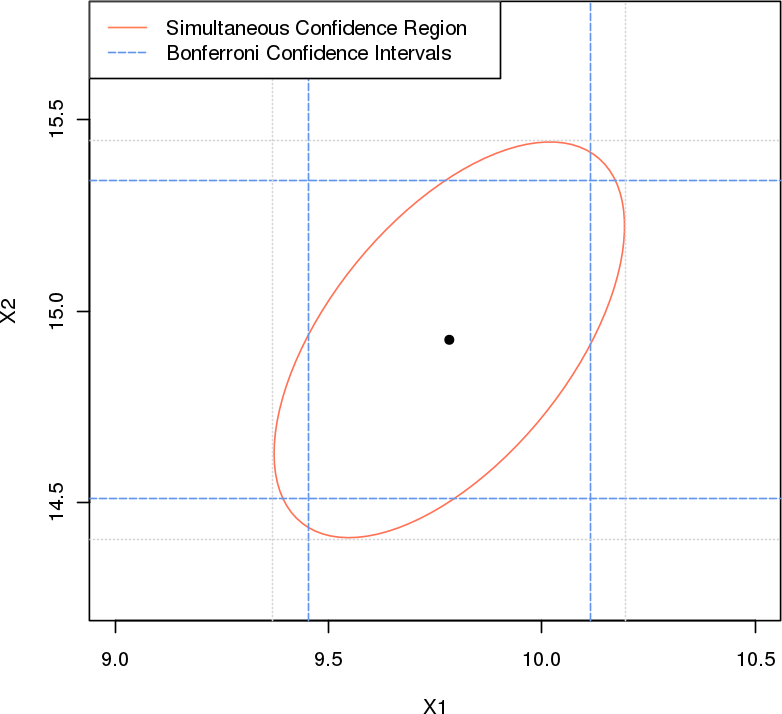
\includegraphics[width=0.44\linewidth]{Images/testA7.png}\quad 
   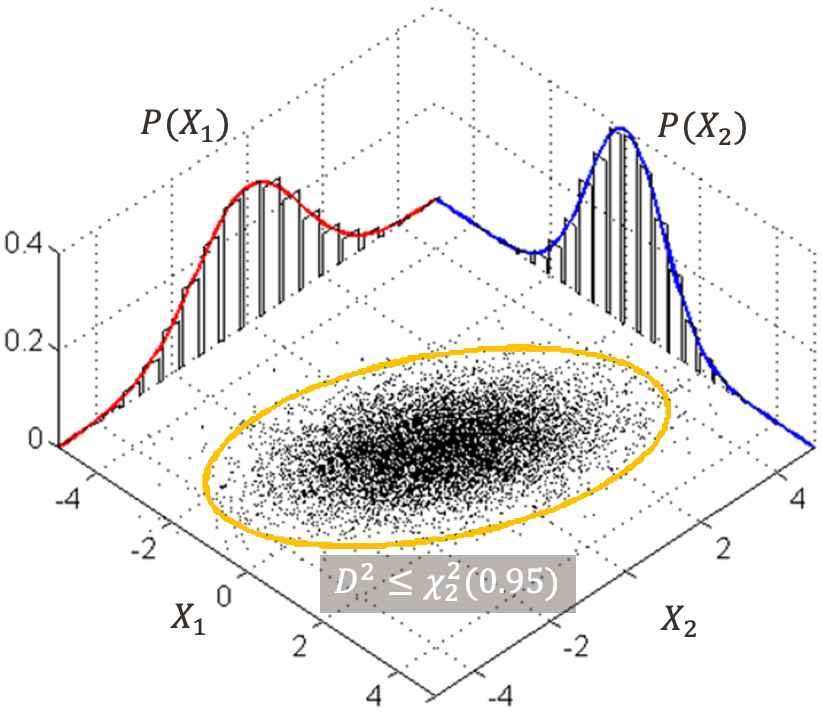
\includegraphics[width=0.48\linewidth]{Images/multivariate.png}

  \caption[\small Confidence regions, Bonferroni and Hotelling simultaneous confidence intervals]{\small $95\%$ confidence ellipse, Bonferroni and Hotelling's ${T}^{2}$ simulatenous confidence intervals for a bivariate normal random sample; showing the  $p=2$ framework [Wikipedia]. }
  \label{fig:testA7}\hrule
\end{figure*}
\begin{enumerate}[noitemsep]
    \item any linear combination of its components are normally distributed;
    \item all subsets of components follow a (modified) multivariate normal distribution;
    \item a diagonal covariance matrix implies the independence of its components;
    \item conditional distributions of components follow a normal distribution, and 
    \item the quantity $(\bm{X}-\bm{\mu})^{\!\top}\bm{\Sigma}^{-1}(\bm{X}-\bm{\mu})$ follows a $\chi^{2}_{p}$.
\end{enumerate}
These properties make the multivariate normal distribution attractive, from a theoretical point of view (if not entirely realistic). For instance, 
\begin{itemize}[noitemsep]
\item using property 1, we can use \textbf{contrasts} to test which components are distinct from the others; \item property 5 is the multivariate analogue of the square of a standard normal random variable $Z\sim N(0,1)$ following a $Z^2\sim \chi^2_1$ distribution;
\item but two univariate normal random variables with zero covariance are not necessarly independent (the joint p.d.f. of two such variables is not necessarily the p.d.f. of a multivariate normal distribution).
\end{itemize}
%A number of univariate approaches generalize nicely. 
\subsection{Hypothesis Testing for Mean Vectors}
When the sample comes from a univariate normal distribution, we can test $$H_{0}: \mu=\mu_{0}\quad\mbox{against}\quad H_{1}: \mu \neq \mu_{0}$$ by using a $t-$statistic. Analogously, if the sample comes from a $p-$variate normal distribution, we can test $$H_{0}: \bm{\mu}=\bm{\mu_{0}}\quad\mbox{against}\quad H_{1}: \bm{\mu} \neq \bm{\mu_{0}}$$ by using \textbf{Hotelling's $\bm{T}^2$ test statistic}
$$
    T^{2}=N\cdot (\bm{\bar{X}}-\bm{\mu})^{\!\top}\bm{S}^{-1}(\bm{\bar{X}}-\bm{\mu})
$$
where $\bm{\bar{X}}$ denotes the \textbf{sample mean}, $\bm{S}$ the \textbf{sample covariance matrix}, and $N$ the sample size. \newpage\noindent  
Under $H_{0}$, $$T^{2}\sim \frac{(N-1)p}{(N-p)}F_{p, N-p}.$$ Thus, we do not reject $H_{0}$ at a significance level of $\alpha$ if 
$$
    N\cdot (\bm{\bar{X}}-\bm{\mu_{0}})^{\!\top}\bm{S}^{-1}(\bm{\bar{X}}-\bm{\mu_{0}}) \leq \frac{(N-1)p}{(N-p)}F_{p, N-p}(\alpha)
$$
and reject it otherwise.
\subsection[Confidence Region and Simultaneous Confidence Intervals]{Confidence Region and Simultaneous Confidence Intervals for Mean Vectors}
In the $p-$variate normal distribution, any $\bm{\mu}$ that satisfies the condition
$$
    N\cdot (\bm{\bar{X}}-\bm{\mu})^{\!\top}\bm{S}^{-1}(\bm{\bar{X}}-\bm{\mu}) \leq \frac{(N-1)p}{(N-p)}F_{p, N-p}(\alpha)
$$
resides inside a $(1-\alpha)100\%$ \textbf{confidence region} (an ellipsoid in this case). \textbf{Simultaneous Bonferroni confidence intervals} with overall error rate $\alpha$ can also be derived, using 
\begin{equation*}
    (\bar{x}_{j}-\mu_{j})\pm t_{N-1}(\alpha/p)\sqrt{\frac{s_{j,j}}{N}} \text{ for $j=1,\ldots, p$}
\end{equation*}
Another approach is to use \textbf{Hotelling's $\bm{T}^2$ simultaneous confidence intervals}, given by 
\begin{equation*}
    (\bar{x}_{j}-\mu_{j})\pm \sqrt{\frac{p(N-1)}{N-p}F_{p,N-p}(\alpha)} \sqrt{\frac{s_{j,j}}{N}} \text{ for $j=1,\ldots, p$}
\end{equation*}
Figure \ref{fig:testA7} shows these regions for a bivariate normal random sample. Notice that the Hotelling's ${T}^{2}$ simultaneous confidence intervals form a rectangle that confines the confidence region, while the Bonferroni confidence intervals are slightly narrower. Given that all the components of the mean vector are correlated (according to a generally non-diagonal covariance matrix), the confidence region should be used if the goal is to study the \textbf{plausibility of the mean vector as a whole}, while Bonferroni confidence intervals may be more suitable when \textbf{component-wise confidence intervals} are of interest. 



%%%%%%%%%%%%%%%%%%%%%%%%%%%%%%%Section 7%%%%%%%%%%%%%%%%%%%%%%%%%%%%%%%%%%% 

